In this section Todo app will be implemented using two standard tools Flutter’s framework provides to handle state: \textbf{InheritedWidget} (or the more advanced \textbf{InheritedModel}) and \textbf{setState}.

\paragraph{State management solution’s introduction} \mbox{}\\ \label{par:todo_app_inherited_widget_introduction}

\textbf{setState} method notify the framework that the internal state of this object has changed.
Whenever you change the internal state of a State object, make the change in a function that you pass to \textit{setState}.\\


\begin{minted}{dart}
setState(() { _myState = newValue; });

\end{minted}

\mbox{}
The provided callback is immediately called synchronously. It must not return a future (the callback cannot be async), since then it would be unclear when the state was actually being set.\\
Calling \textit{setState} notifies the framework that the internal state of this object has changed in a way that might impact the user interface in this subtree, which causes the framework to schedule a build for this State object.\\
If you just change the state directly without calling \textit{setState}, the framework might not schedule a build and the user interface for this subtree might not be updated to reflect the new state.\\
\textbf{Inherited widget} are a base class for widgets that efficiently propagate information down the tree.
To obtain the nearest instance of a particular type of inherited widget from a build context, use \textit{BuildContext.dependOnInheritedWidgetOfExactType}.
Inherited widgets, when referenced in this way, will cause the consumer to rebuild when the inherited widget itself changes state.
The convention is to provide a static method \textit{of} on the InheritedWidget which does the call to \textit{BuildContext.\textit{dependOnInheritedWidgetOfExactType}}. This allows the class to define its own fallback logic in case there isn't a widget in scope.
An InheritedWidgets is not intended to be used as the base class for models whose dependents may only depend on one part or "\textit{aspect}" of the overall state. Indeed inherited widget's dependents are unconditionally rebuilt when the inherited widget changes. \\


\textbf{InheritedModel} widget is similar except that dependents aren't rebuilt unconditionally.
Widgets that depend on an InheritedModel qualify their dependence with a value that indicates what "\textit{aspect}" of the model they depend on. When the model is rebuilt, dependents will also be rebuilt, but only if there was a change in the model that corresponds to the aspect they provided.
\paragraph{Base functionalities} \mbox{} \\
\label{par:todo_app_inherited_widget_base_app}
Here stars the implementation of the base functionalities exposed in Subsection \ref{subsec:base_functionalities}.
\subparagraph{Core state}\mbox{}\\
\label{subpar:todo_app_inherited_widget_core_state}
In order to use InheritedWidget's functionalities a new class must be defined and extended with InheritedWidget class. This new class will contain the state ,or part of it. For our purpose a single class will be enough to contain all the state. This new class is called \textit{TodoInheritedData}.

\captionof{listing}{Todo app - extension to InheritedWidget} \mbox{}

\begin{minted}{dart}
class TodoInheritedData extends InheritedWidget{
\end{minted}
\mbox{}

The accessible state is composed by: a list of Todos, a VisibilityFilter , a Int for the stats ( for conciseness it will represent the number of completed todos) and filtered list of todos that will contain the todos matching the filter. Inside the constructor, final variables are initialized with the corresponding arguments and \textit{stats} and \textit{filteredTodos} variables are computed. \textit{filterTodos} function is just a function that takes the full list of todos and a filter and returns the filtered list. Important to notice is the fact that a \textit{child} widget must be also provided in the constructor. This is because TodoInheritedData is nothing else than a widget itself that wraps data and make it accessible down the tree.

\mbox{}\\
\captionof{listing}{Todo app - TodoInherited data implementation} \mbox{}

\begin{minted}{dart}

class TodoInheritedData extends InheritedWidget{
  final List<Todo> todos;
 final List<Todo> filteredTodos;
 final VisibilityFilter filter;
 final int stats;
 
TodoInheritedData(
    { 
    Key? key,
    required this.todos,
    required this.filter,
    required Widget child})
    : stats = todos.length,
      filteredTodos = filterTodo(todos, filter),
      super(child: child, key: key);
}
\end{minted}


TodoInheritedData widget is stateless. It cannot be changed (every value is final) ,instead , a new TodoInheritedData widget must be provided when a data change occurs. 
The \textit{updateShouldNotify }function must be overridden inside TodoInheritedData class. This function belongs to the InheritedWidget class and its reimplementation is mandatory. It helps to avoid useless UI rebuilding when a new state ,without actual data changes , occurs. Once a TodoInheritedData element is replaced with a new one, the new element takes care to call the \textit{updateShouldNotify }method and to decide whether is necessary to notify changes in the subtree. If the method returns \textit{true }the subtree is rebuilt, if returns \textit{false} ,instead, it is not.
\mbox{}\\

\captionof{listing}{Todo app - InheritedWidget -updateShouldNotify method override} \mbox{}

\begin{minted}{dart}

@override
bool updateShouldNotify(TodoInheritedData oldWidget) {
  return !listEquals(oldWidget.filteredTodos, filteredTodos);
}
\end{minted}

\textit{listEquals }function takes as parameters the old \textit{filteredTodos} list ,contained in the \textit{oldWidget} argument, and the new filteredTodos list and compare them element by element checking if changes occurs. In case no changes were performed it returns \textit{true} and leads the \textit{updateShouldNotify }function to return \textit{false}. In this way the entire subtree is not rebuilt.\\
InheritedWidget class requires also the \textit{of} method override. The \textit{of }method makes the instance of the TodoInheritedData class accessible down the tree. It is a static method that can be called without istantiating any TodoInheritedData object and returns the instance of the nearest TodoInheritedData widget up in the tree. It extracts the instance from the current \textit{context} object using the method called \textit{dependOnInheritedWidgetOfExactType} provided by the framework. In case no TodoInheritedData instance is found it raises an error.


\captionof{listing}{Todo app - InheritedWidget - TodoInheritedData of method override} \mbox{}
\begin{minted}{dart}

static TodoInheritedData? of(BuildContext context) {
 final TodoInheritedData? result = context.dependOnInheritedWidgetOfExactType<TodoInheritedData>(); 
assert(result != null, 'No TodoInheritedData found in context');
return result;
}
\end{minted}


TodoInheritedData widget can be now used it in a stateful widget. This new statefull widget is called \textit{TodoProvider.}

\captionof{listing}{Todo app - InheritedWidget - TodoProvider implementation} \mbox{}

\begin{minted}{dart}

class TodoProvider extends StatefulWidget {
  const TodoProvider({Key? key, required this.child}) : super(key: key);

  final Widget child;

  @override
  _TodoProviderState createState() => _TodoProviderState();
}

class _TodoProviderState extends State<TodoProvider> {
  List<Todo> todos = [];
  VisibilityFilter filter = VisibilityFilter.all;

@override
Widget build(BuildContext context) {
  return TodoInheritedData(
    todos: todos,
    filter: filter,
    child: widget.child,
  );
}
\end{minted}

Note that the VisibilityFilter ,\textit{filter}, is set as \textit{all} by default.
In the statefull widget's \textit{init} method , todos are fetched from the repository and pushed inside the \textit{todos} variable using the \textit{setState} method.
\mbox{}\\

\captionof{listing}{Todo app - InheritedWidget - TodoProvider 's init method implementation} \mbox{}

\begin{minted}{dart}

@override
void initState() {
  TodoRepository.loadTodos().then((todos) {
    setState(() {
      this.todos = todos;
    });
  });
  super.initState();
}
\end{minted}

\textit{loadTodos }is a TodoRepository’s async function that simulate the retrieval of the todos from a database as defined in the paragraph \ref{par:todo_app_models_and_repository}.

At this point our TodoProvider widget can be incorporated as the parent of the Scaffold widget in the HomePage. The usage of the Builder widget is due to the fact that the instante of TodoInheritedData is accessible only in a context where a TodoProvider is already present. In other word TodoProvider’s data cannot be accessed in the same \textit{build } method where it was instantiated into. Two options are possible; creating a separated file where to put our Scaffold or use a Builder widget that takes the current context and creates another with the TodoProvider widget.
\mbox{}\\


\captionof{listing}{Todo app - InheritedWidget - data's injection in the tree} \mbox{}

\begin{minted}{dart}

@override
Widget build(BuildContext context) {
  return TodoProvider(
    child: Builder(
      builder: (context) {
        return Scaffold();      }
  );
}
\end{minted}

\subparagraph{The TodoView component}\mbox{}\\
\label{subpar:todo_app_inherited_widget_todoview_component}
TodoView component can now be populated. Its implementation can be found in paragraph \ref{par:todo_app_components} in subsection \ref{subsec:todo_app_shared_project_structure}. It is a stateless widget that looks up for the \textit{filteredTodos} list, contained in the TodoInheritedData widget. It uses the \textit{of} method ,defined here RIFERIMENTO, to access the nearest TodoInheritedData instance. Then, it uses the list to populate the ListView widget. 
\mbox{}\\


\captionof{listing}{Todo app - InheritedWidget - TodoView implementation} \mbox{}

\begin{minted}{dart}

class TodoView extends StatelessWidget {

  const TodoView({Key? key}) : super(key: key);

  @override
  Widget build(BuildContext context) {
    print("Building TodoView");

    final List<Todo> filteredTodos = TodoInheritedData.of(context).filteredTodos;

    return ListView.builder(
      itemCount: filteredTodos.length,
      itemBuilder: (context, index) {
        return TodoItem(
          todo: filteredTodos.elementAt(index),
        );
      },
    );
  }
}
\end{minted}


\subparagraph{The VisibilityFilterSelector component}\mbox{}\\
\label{subpar:todo_app_inherited_widget_visibilityfiltercomponent_component}
At this point we got a single page (Homepage) that uses a TodoView widget to show the \textit{filteredTodos} list contained in the TodoInheritedData widget. When the application starts , and empty page appears (todo are empty at the beginning) and then ,after few seconds , a list of todos, with their names, descriptions and completions, is shown. The list of filtered todos can be visualized , but is not interactable yet. 
In the HomePage’s AppBar, a VisibilityFilterComponent is already set up as defined RIFERIMENTO. Its DropdownButton’s \textit{value} field is set looking up for the \textit{filter} value in the TodoInheritedData widget. Then , the \textit{items} field is filled with a list of DropdownMenuItem widgets that comes from the mapping of all possible VisibilityFilter values to DropdownMenuItem widgets.
\mbox{}\\


\captionof{listing}{Todo app - InheritedWidget - VisibilityFilterComponent implementation} \mbox{}

\begin{minted}{dart}
class VisibilityFilterComponent extends StatelessWidget {

  const VisibilityFilterComponent(
      {Key? key})
      : super(key: key);

  @override
  Widget build(BuildContext context) {
    print("Building Visibility filter");
    VisibilityFilter filter= TodoInheritedData.of(context).filter;
    return DropdownButton<VisibilityFilter>(
      value: filter,
      items: VisibilityFilter.values.map((filter) {
        return DropdownMenuItem<VisibilityFilter>(
            child: Text(describeEnum(filter)), value: filter);
      }).toList(),
      onChanged: (filter) {
        
      },
    );
  }
}
\end{minted}

The \textit{onChanged  }field must be populated with a function that takes as single argument a VisibilityFilter value. This function is called when a DropdownMenuItem is tapped by the user. It contains ,in its argument, the tapped DropdownMenuItem's filter value.  We want this function to change the state contained in the TodoInheritedData widget (the \textit{filter} variable) when fired. In order to do so , a state changing function must be provided by the TodoInheritedData widget to be accessed ,and called, by other widgets. As we mentioned earlier, TodoInheritedData widget contains only final fields and should never be modified. It is not possible ,indeed, to directly change the values inside the TodoInheritedData widget. For this reason , just adding a new function inside the TodoInheritedData widget ,to perform the change, is not a solution. Indeed, trying to change a part of the state, inside this ipotetic function, will generate an error at compile time (final variable cannot be set outside constructor). A completly new TodoInheritedData widget ,indeed, should be created. The TodoInheritedData widget is created in the TodoProvider widget, when the \textit{build} method runs, using its local variables \textit{todos }and \textit{filter}. In order to generate a new TodoInheritedData widget, is sufficient to change the TodoProvider widget's local state ,using the \textit{setState} method. This will cause the \textit{build} method to run again with the new values and generate a new TodoInheritedData widget. At this point should be clear that the state changing function comes from the TodoProvider widget. This function , once called, changes the local state of the TodoProvider stateful widget generating a new state for the application.\\
In pratice ,a new function ,called \textit{onChangeFilter}, is added inside the TodoProvider widget. This function takes a VisibilityFilter value as parameter and set the  value of TodoProvider's \textit{filter} variable using \textit{setState} method. 

\mbox{}\\


\captionof{listing}{Todo app - InheritedWidget - TodoProvider's onChangeFilter implementation} \mbox{}

\begin{minted}{dart}
void onChangeFilter(VisibilityFilter filter) {
  setState(() {
    this.filter = filter;
  });
}
\end{minted}

Once called, being the state (the part concerning the filter) changed, another run of the \textit{build} method is performed. As a conseguence the TodoInheritedData widget ,present in the tree, is replaced with the new one.
However, widgets access the state through the TodoInheritedData widget and not through the TodoProvider widget. For this reason,
the \textit{onChangeFilter   }function must be provided to the TodoInheritedData to make it accessible in the subtree. A new parameter is added in the TodoInheritedData class, tough.


\mbox{}\\

\captionof{listing}{Todo app - InheritedWidget - TodoInheritedData widget expansion}
\begin{minted}{dart}
class TodoInheritedData extends InheritedWidget {
  {...}
  final void Function(VisibilityFilter) onChangeFilter;
  {...}
\end{minted}

The \textit{onChangeFilter} function is then passed to the TodoInheritedData widget on its creation.
 
\captionof{listing}{Todo app - InheritedWidget -onChangeFilter function injection into TodoInheritedData widget}

\begin{minted}{dart}
@override
Widget build(BuildContext context) {
  return TodoInheritedData(
    todos: todos,
    onChangeFilter: onChangeFilter,
    filter: filter,
    child: widget.child,
  );
}

\end{minted}
 
Now that the \textit{onChangeFilter   }function is accessible down in the tree, it can be called in the \textit{onChange }field of the DropdownButton widget, inside the VisibilityFilterSelector component.
\mbox{}\\


\captionof{listing}{Todo app - InheritedWidget -  DropdownButton's onChanged field implementation}

\begin{minted}{dart}
onChanged: (filter) {
  TodoInheritedData.of(context).onChangeFilter(filter!);
},
\end{minted}

It is now possible to apply different filters to the list of todos in the Homepage. 


\subparagraph{The TodoItem component}\mbox{}\\
\label{subpar:todo_app_inherited_widget_todoitem_component}
TodoItem widget is stateless for the moment. It that take as paramenter a Todo and takes care of displaing it as defined in \ref{subsec:todo_app_shared_project_structure}. TodoItem does not really access the state to read values. The todo to be displayed is ,indeed, passed by the parent widget (the TodoView). However, the TodoItem widget needs to "write" the state, once the checkbox is tapped. For the moment the Checkbox widget ,inside every TodoItem, is just showing their  todo's completion but its \textit{onChange   }function is still empty and does nothing when tapped. When the CheckBox is tapped a change in the corresponding Todo’s \textit{completed }field should be fired and a rebuild of the TodoItems performed. In order to do so, TodoIhneritedData should provide a state changing function, down the tree, that allow to perform this change. The process to be performed and the reasoning is the same exposed in the previous paragraph: paragraph \ref{subpar:todo_app_inherited_widget_visibilityfiltercomponent_component} . Going back again to the TodoProvider stateful widget a function ,called \textit{onSetCompleted  }, is added . This function takes as parameter the id of the todo to be changed and the new value for the \textit{completed }field.
\mbox{}\\


\captionof{listing}{Todo app - InheritedWidget -  TodoProvider widget \textit{onSetCompleted} function implementation}

\begin{minted}{dart}
void onSetCompleted(int id, bool completed) {
  assert(todoExists(id) != null, 'No todo with id : \$id');

  setState(() {
    todos = todos.map((e) {
      if (e.id == id) {
        return Todo(
            id: id,
            name: e.name,
            description: e.description,
            completed: completed);
      } else {
        return e;
      }
    }).toList();
  });
}
\end{minted}

In the \textit{onSetCompleted }function the \textit{todos }list is scanned using a map. Once the todo with the corresponding id is found, its \textit{completed }value is modified to the new value. Calling the \textit{onChangeFilter }method on the TodoProvider stateful widget will cause the \textit{build}  method to run again and to create another TodoInheritedData. As usual , the function is passed from the TodoProvider widget to the TodoInheritedData widget on its creation. In this way the function is now accessible down the tree. It is now possible to call it inside the onChanged method of the TodoItem's Checkbox.


\mbox{}\\


\captionof{listing}{Todo app - InheritedWidget -  TodoItem's Checkbox \textit{onChanged} field implementation}

\begin{minted}{dart}
Checkbox(
value: todo.completed,
    onChanged: (value) {
    	TodoInheritedData.of(context).onSetCompleted(todo.id, value!);
}),
\end{minted}

\mbox{}\\


At this point is possible to visualize the \textit{filteredTodos} list, change the filter and update Todo’s \textit{completed }field.


\subparagraph{The Stats component}\mbox{}\\
\label{subpar:todo_app_inherited_widget_stats_component}

Stats widget is stateless. It just needs to read the state, the part concerning the stats. The nearest instance of the TodoInheritedData widget is retrieved using the \textit{of} method and used to fill the Text widget.


\mbox{}\\

\captionof{listing}{Todo app - InheritedWidget -  Stats component implementation}

\begin{minted}{dart}
class Stats extends StatelessWidget {
  const Stats({Key? key}) : super(key: key);

  @override
  Widget build(BuildContext context) {
    print("Building Stats");

    return Center(
        child: Text(TodoInheritedData.of(context).stats.toString()));
  }
}
\end{minted}


\subparagraph{The TabSelector component}\mbox{}\\
\label{subpar:todo_app_inherited_widget_tabselector_component}
The state of the tab is just one variable and is relate to the HomePage only. An important aspect of the state management is that not all the state must be mandatory contained in the tool the various solutions propose. Sometimes, indeed, for the parts of the state that can be refered as "local" ,meaning that are relative to a small part of the application only, is not necessary to use overcomplicated strucuture. Using a state management solution does not mean that every part of the state must be handled with it. It is better to keep things simple and use the tools that most adapt to the specific scenario.
For example, there are two ways to implement the TabSelector widget: use \textit{setState} and stateful widget or use InheritedWidgets. The simpler one is to use setState as proposed RIFERIMENTO for more than one reason. First, it is a good practice to keep the global state of the application as small and clean as possible. The more it gets big and complicated the messier become to avoid bugs. Second, it is simpler , in pratice, to create a local variable and hadle it with setState and stateful widgets instead of adding it to the TodoInheritedData widget and to TodoProvider widget and then access it in the HomePage. The HomePage is already a stateful widget and is built using the \textit{tab }variable. It is sufficient to add a new function to change the tab value from \textit{todos} value to \textit{stats} value and the other way around. This new function ,called \textit{onTabChange}, takes a int value as parameter and uses the \textit{setState} method to set the \textit{tab} variabile with the corresponding TabState value. However, the function needs to be accessible in the TabSelector widget and not in the HomePage. The easiest way is to pass the function ,to the TabSelector widget ,as parameter.

Then a new TabState variable is created in the HomePage called \textit{tab} and set as TabState.todos by default. A function called \textit{onTabChange} will call the \textit{setState} method modifying the tab value and causing the \textit{build} method to run again. 
\mbox{}\\


\begin{minted}{dart}
TabState tab = TabState.todos;

void onTabChange(int index) {
 setState(() {
   tab = TabState.values.elementAt(index);
 });
}
\end{minted}

\textit{tab} value and \textit{onTabChange} function are now passed to the TabSelector component as parameters and used to populate the BottomNavigationBar widget.

\mbox{}\\


\begin{minted}{dart}
class TabSelector extends StatelessWidget {
  final TabState currTab;
  final Function(int) onTabChange;

  const TabSelector(
      {Key? key, required this.currTab, required this.onTabChange})
      : super(key: key);

  @override
  Widget build(BuildContext context) {
    print("Building Tab Selector");

    return BottomNavigationBar(
      currentIndex: TabState.values.indexOf(currTab),
      onTap: onTabChange,
      items: TabState.values
          .map((tab) => BottomNavigationBarItem(
                label: describeEnum(tab),
                icon: Icon(
                  tab == TabState.todos ? Icons.list : Icons.show_chart,
                ),
              ))
          .toList(),
    );
  }
}

\end{minted}

 
At this point all the basic functionalities have been implemented. \\
Down below some images taken from an execution of the application. Six todos are randomly created and only two of them are marked as completed.

\begin{figure}[H]
    \centering
    \subfloat[todos tab runtime UI.\label{fig:todos_tab_UI}]{
        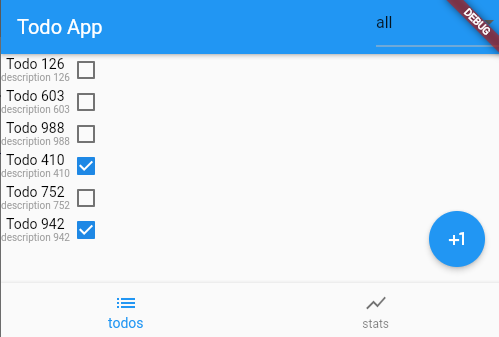
\includegraphics[scale=0.6]{Images/shot_runtime_todoapp.png}
    }
    \quad
    \subfloat[todos tab runtime widget tree.\label{fig:todos_tab_tree}]{
        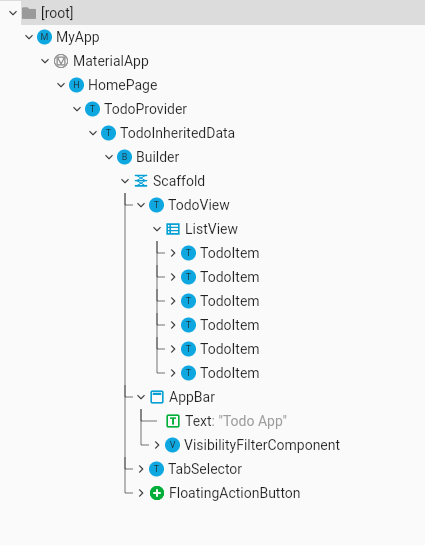
\includegraphics[scale=0.6]{Images/tree_structure_on_HomePage_todos.png}
    }
    \caption{Show the runtime Widget's tree and UI when visualizing todos tab.}
    \label{fig:todos_tab}
\end{figure}
Figure~\ref{fig:todosTabUI} shows how the application UI looks like after few seconds from the start. Figure~\ref{fig:todosTabTree} show the widgets tree related with the run.
\begin{figure}[H]
    \centering
    \subfloat[stats tab runtime UI.\label{fig:stats_tab_UI}]{
        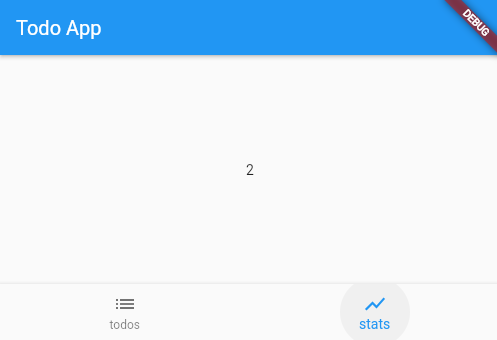
\includegraphics[scale=0.6]{Images/shot_runtime_todoapp_stats.png}
    }
    \quad
    \subfloat[stats tab runtime widget tree.\label{fig:stats_tab_tree}]{
        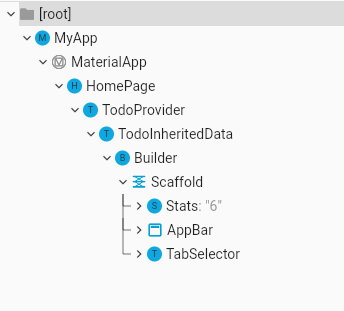
\includegraphics[scale=0.6]{Images/tree_structure_on_HomePage_stats.png}
    }
    \caption{Show the runtime Widget's tree and UI when visualizing stats tab.}
    \label{fig:stats_tab}
\end{figure}
Figure~\ref{fig:todosTabUI} shows how the application UI looks like after the user taps on the TabSelector's stats button. Figure~\ref{fig:todosTabTree} show the widgets tree related with the run after the button is clicked.\\
\\
Time spent: 2-3 hours\\
Lines of code written/updated: 86\\
Classes/widget created: 2 ( TodoInheritedData class and TodoProvider widget)\\



\paragraph{Features addition} \mbox{} \\
\label{par:feature_addition_inherited_widget}
Here stats the development part where the todo addition feature and the todo update feature are implemented.

\subparagraph{Todo addition feature} \mbox{} \\
\label{subpar: todo_addition_feature_inherited_widget}
A new function must be implemented in the TodoProvider widget and passed to the TodoInheritedData widget. This new function will be called \textit{onAddTodo} and will take two parameters (name and description).
\mbox{}\\


\begin{minted}{dart}

void onAddTodo(String name, String desc) {
  Random rand = Random();
  List<int> ids = todos.map((e) => e.id).toList();
  int newId = rand.nextInt(1000) + 2;
  while (ids.contains(newId)) {
    newId = rand.nextInt(1000) + 2;
  }
  Todo newTodo = Todo(
      id: newId,
      name: name,
      description: desc+ " " + newId.toString(),
      completed: false);
  List<Todo> newList = List.from(todos);
  newList.add(newTodo);
  setState(() {
       todos = newList;
  });
}
\end{minted}

After generating a new unique id it creates a new Todo object called \textit{newTodo }with the \textit{completed }field set to \textit{false }. Adding the new Todo to the TodoProvider’s state \textit{todos }list requires a bit of workaround. The state of a stateful widget is immutable. It can only be changed by the \textit{setState } method. Unfortunately, the method \textit{add} for lists is of type void and do not return a new list but instead add the new value to the existing one. For this reason directly calling the \textit{add} method to the TodoProvider’s local lists \textit{todos }will have no effect. That list is immutable and cannot be changed.
TodoProvider’s \textit{todos }list must be completely replaced with a new list containing also the new todo. First a new temporary list called \textit{newList} is created and populated with the element present in the \textit{todos }list. Then the \textit{newTodo }is added to this \textit{newList} list. At this point is sufficient to replace the \textit{todos }list with the new one inside the \textit{setState} method.
To make this new function accessible down the tree is sufficient to add a new field in the TodoInheritedData (called onAddTodo) widget and pass the function on creation.
\mbox{}\\


\begin{minted}{dart}

class TodoInheritedData extends InheritedWidget {
  {...}
  final void Function(String,String) onAddTodo;

  {...}

@override
Widget build(BuildContext context) {
  return TodoInheritedData(
    todos: todos,
    onChangeFilter: onChangeFilter,
    onAddTodo: onAddTodo,
    onSetCompleted: onSetCompleted,
    filter: filter,
    child: widget.child,
  );
}
\end{minted}

In the AddTodoPage a TextButton has been already set up and is ready to call this function once tapped. However, there is a small inconvenient. The AddTodoPage is accessed by pushing on top of the HomePage another route as shown in figure \ref{fig:addTodoPage}. 

\begin{figure}[H]
    \centering
    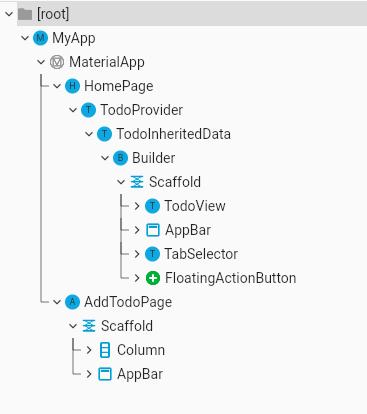
\includegraphics[width=0.6\textwidth]{Images/tree_structure_on_AddTodoPage.png}
    \caption{Show the tree structure after the FloatingActionButton in the HomePage is tapped.}
    \label{fig:add_todo_page_tree_structure}
\end{figure}


In this new scope the Scaffold widget inside the AddTodoPage become the root of the tree of the current route. In other words, the AddTodoPage is not a part of the subtree of the HomePage but is a standalone tree instead. There is no instance of TodoProvider as ancestor of the AddTodoPage Scaffold widget and so it is not possible to call the \textit{of} method as before. Indeed calling the \textit{of} method in a context where a TodoProvider is not present will cause the line
\mbox{}\\


\begin{minted}{dart}

assert(result != null, 'No TodoInheritedData found in context');
\end{minted}

inside it to return \textit{false} and rise a runtime error. The easiest method to proceed is to pass the \textit{onAddTodo} function as a parameter to the AddTodoPage when we push it on top of the HomePage. So a new parameter called \textit{addTodoCallback }is added to the AddTodoPage 
\mbox{}\\


\begin{minted}{dart}

class AddTodoPage extends StatefulWidget {

  final void Function(String,String) addTodoCallback;
    {. . .}
\end{minted}

And the material app is notified about the necessity of this new argument in the AddTodoPage creation.
\mbox{}\\


\begin{minted}{dart}

routes: {
{. . .}
  "/addTodo": (context) => AddTodoPage(
      addTodoCallback: ModalRoute.of(context)!.settings.arguments
          as Function(String, String)),
},

\end{minted}

At this point the \textit{onChange  }function of the TextButton inside the AddTodoPage can finally be populated as follow
\mbox{}\\


\begin{minted}{dart}

TextButton(onPressed: () {
  widget.addTodoCallback(textControllerName.text,textControllerDesc.text);
  Navigator.pop(context);
}
\end{minted}

The current route (AddTodoPage) is also popped after the todo creation, and the HomePage is rebuilt (by the fact the TodoInheritedData changed).\\
\\
\textbf{Time spent: 20-30 minutes\\
Lines of code written/updated: 24\\ 
Classes/widget created: 0\\
}
\subparagraph{Todo updating feature} \mbox{} \\
\label{subpar:todo_updating_feature_inherited_wdiget}
First thing is to create and make the \textit{onUpdateTodo } feature/function accessible down the tree. A new function must be implemented in the TodoProvider widget and passed to the TodoInheritedData widget. This new function will be called \textit{onUpdateTodo } and takes three arguments: the id of the todo to be updated, the \textit{newName } that should be set and the \textit{newDesc}.

\mbox{}\\


\begin{minted}{dart}

void onUpdateTodo(int id, String newName,String newDesc) {
  assert(todoExists(id) != null, 'No todo with id : \$id');
  List<Todo> newTodosList = todos.map((element) {
    if (element.id == id) {
      return Todo(
          completed: element.completed,
          description: newDesc,
          name: newName,
          id: element.id);
    } else {
      return element;
    }
  }).toList();
  setState(() {
    todos = newTodosList;
  });
}

\end{minted}


It first checks if a todo matching the id exists. Then, for the same immutability concept we dealt with when we spoke about the \textit{onAddTodo} feature, a \textit{newTodosList }is created and populated with the elements inside the \textit{todos }list. Moreover, the todo with the corresponding id is update with the new name and new description. Finally, the \textit{todos }list in the TodoProvider stateful widget is overridden with the \textit{newTodosList }using the \textit{setState} method.
This new \textit{onUpdateTodo} method is then made accessible down the tree adding it to the TodoInheritedData.
\mbox{}\\


\begin{minted}{dart}

class TodoInheritedData extends InheritedWidget {
  ...
  final void Function(int, String,String) onUpdateTodo;
  ...


@override
Widget build(BuildContext context) {
  return TodoInheritedData(
    todos: todos,
    onChangeFilter: onChangeFilter,
    onAddTodo: onAddTodo,
    onSetCompleted: onSetCompleted,
    onUpdateTodo: onUpdateTodo,
    filter: filter,
    child: widget.child,
  );
}
\end{minted}

For the same problem faced during the implementation of the todo addition feature also in this case the \textit{onUpdateTodo } function must be passed to the new route (no TodoProvider present in this context) as parameter. A new variable is added to the UpdateTodoPage ,beside the already existent one, called \textit{callback }. This new variable will be a Function taking two Strings as arguments (the id will be already set up by the calling page).

\mbox{}\\


\begin{minted}{dart}

class UpdateTodoPage extends StatefulWidget {
  final Todo todo;
  final void Function(String,String) callback;
 \end{minted}
 

Inside the \textit{onTap }function of the TodoItem's InkWell widget the route UpdateTodoPage will be pushed but first a container for arguments must be set up. Indeed, Flutter Navigator allows to pass only a single object as argument between routes. In this case not only the \textit{onUpdateTodo} function must be passed to the new route but also some information about the Todo itself. For this reason a wrapper class is created with the name \textit{UpdateTodoPageArguments }.
\mbox{}\\


\begin{minted}{dart}

class UpdateTodoPageArguments {
  final Todo todo;
  final void Function(String ,String) updateState;

  UpdateTodoPageArguments({required this.todo, required this.updateState});
}
\end{minted}

and inside the InkWell’s \textit{onTap }function will be used to create a container for the arguments.
\mbox{}\\


\begin{minted}{dart}

Navigator.pushNamed(context, "/updateTodo",
    arguments: UpdateTodoPageArguments(
        todo: todo,
        updateState: (String newName,String newDesc) {
          TodoInheritedData.of(context, aspect: 0)
              .onUpdateTodo(todo.id, newName,newDesc);
        }));
\end{minted}

A further change must be done in the MaterialApp’s  “/updateTodo” route to populate the field of the UpdateTodoPage correctly.
\mbox{}\\


\begin{minted}{dart}

routes: {
  "/": (context) => const HomePage(),
  "/updateTodo": (context) => UpdateTodoPage(
        todo: (ModalRoute.of(context)!.settings.arguments
                as UpdateTodoPageArguments)
            .todo,
        callback: (ModalRoute.of(context)!.settings.arguments
                as UpdateTodoPageArguments)
            .updateState,
      ),
\end{minted}

Now that the \textit{onUpdateTodo } function is set up and correctly passed to the UpdateTodoPage is the time to call it inside the TextButton \textit{onPressed  }field like this
\mbox{}\\


\begin{minted}{dart}

TextButton(onPressed: () {

  widget.callback(textControllerName.text,textControllerDesc.text);
  Navigator.pop(context);
},
\end{minted}

Once pressed the UpdateTodoPage will be popped, and the HomePage rebuilt to show the actual changes in the \textit{todos }list.\\
\\
\textbf{Time spent: 20-30 minutes\\
Lines of code written/updated: 43\\ 
Classes/widget created: 1 for arguments between routes\\
}

\subparagraph{Render optimizations} \mbox{} \\
\label{subpar:render_optimizations_inherited_widget}
This was a pretty hard task. I spent some hour trying to figure out how make , when a single todo update occurs, rebuild the TodoItem only instead of the entire TodoView. Then I realized that it was just not feasible using InheritedWidgets. InheritedWidget indeed do not offer this possibility at all. Every widget in the TodoProvider’s subtree that access the state is registered as listener for state changes and once a state change occurs there are only two possibilities: notify all those widgets and rebuild them or not. In other words when a state change occurs and must be visualized the entire TodoProvider’s subtree must be rebuilt unconditionally. Flutter framework however offers a particular widget called InheritedModel to handle this scenario. InheritedModel work as InheritedWidget except for the fact that when a widget access the state (calling the \textit{of} method) it must provide also a new additional parameter called \textit{aspect}. \textit{Aspect} can be whatever object, for example a String or a Int, but also a more complex data structure. The \textit{aspect} parameter identifies on which part (or parts) of the state the widget is registering to. \\
First thing to do is to substitute the extension to InheritedWidget with InheritedModel in the
TodoInheritedData class (in the todo\_provider.dart file).
\mbox{}\\


\begin{minted}{dart}

class TodoInheritedData extends InheritedWidget {
\end{minted}

to
\mbox{}\\


\begin{minted}{dart}

class TodoInheritedData extends InheritedModel<int> {
\end{minted}

I decided to use Ints to identify aspects. In particular, widgets that need to rebuild on \textit{filteredTodos} list structure change will register to aspect identified with the number 0. Widgets that do never need to rebuild will register to aspect identified with number 1. Widgets that need to rebuild when a change in a specific Todo with id n occurs will register to the aspect identified with the number n. (no Todos will have id with value 0 or 1. This is a convention I used to keep things simple. Other more complex structure could be used to avoid this behaviour). With \textit{filteredTodos} structure I mean the length of the list. TodoView indeed should be entirely rebuilt only when a Todo is added or removed from the list changing its length. No todos replacement is considered by the fact that a replacement should be split into two separated actions ; a deletion and an insertion.
At this point the method \textit{of} should be updated taking into account also the aspect parameter. Morevover, the \textit{result} variable should be populated with the \textit{inheritedFrom  }static method belonging to the InheritedModel class instead of the \textit{dependOnInheritedWidgetOfExactType} method belonging to InheritedWidget class.
\mbox{}\\


\begin{minted}{dart}

static TodoInheritedData of(BuildContext context, {required int aspect}) {
  final TodoInheritedData? result =
      InheritedModel.inheritFrom<TodoInheritedData>(context, aspect: aspect);
  assert(result != null, 'No TodoInheritedData found in context');
  return result!;
}
\end{minted}

Now all the lines of code that access the state with the \textit{of} method must be changed taking into account the new implementation and the new \textit{aspect} argument in this way
\mbox{}\\


\begin{minted}{dart}

TodoInheritedData.of(context, aspect: aspect)
\end{minted}

In particular the TodoView widget will pass as aspect the number 0 declaring that should be notified (and rebuild) only when a \textit{filteredTodos}’s structure change occurs.
Instead TodoItem widgets will pass the corresponding Todo’s \textit{id} as aspect parameter.
Now that every widget is registered only to the desired aspect of the data, is necessary to “teach” the TodoInheritedData to recognize which aspect of the data actually changed when a state change occurs. To do so InheritedModel provides a method called \textit{updateShouldNotifyDepenedent} that is just like the InheritedWidget’s one \textit{updateShouldNotify }but this time takes as argument also a Set of ints called \textit{dependencies }  (aspects). This method is called once for every widget that registered to state changes and the \textit{dependencies }  variable will contains all aspects the widgets registered to (only one for widget in our case). As follow the implementation of the method:
\mbox{}\\


\begin{minted}{dart}

@override
bool updateShouldNotifyDependent(
    TodoInheritedData oldWidget, Set<int> dependencies) {
  int currLen = filteredTodos.length;
  int prevLen = oldWidget.filteredTodos.length;
  bool structureRebuildlen = (dependencies.contains(0) && currLen != prevLen);
  if (structureRebuildlen == true) {
    return true;
  } else {
    List<int> currIds = filteredTodos.map((todo) => todo.id).toList();
    List<int> prevIds =
        oldWidget.filteredTodos.map((todo) => todo.id).toList();
    bool sameIds = listEquals(currIds, prevIds);
    bool structureRebuildcomp = (dependencies.contains(0) && !sameIds);
    if (structureRebuildcomp == true) {
      return true;
    } else {
      List<bool> components = [];
      for (var element in filteredTodos) {
        components.add(dependencies.contains(element.id) &&
            !oldWidget.filteredTodos.contains(element));
      }
      bool res = components.fold(false,
          (bool previousValue, bool element) => previousValue || element);
      return res;
    }
  }
}
\end{minted}

This was tough to code but in the end worked well for the purpose. The method's pseudocode is presented down below. 

\begin{minted}{dart}
if( widgetRegisteredForStructureChange && strucutureChangeOccured){
        return true;
    }else{
        if( widgetRegisteredForSpecificTodoChange && thatTodoChanged){
            return true;
            }else{
                return false;
    }
}
\end{minted}


At this point the TodoItem’s checkbox is tapped just the TodoItem is rebuilt. No visual changes are shown, however. The widget will rebuild with the same information as before and this is due to the fact that the \textit{build} method refers to the local TodoItem's Todo variable. This variable is populated on the TodoItem creation and cannot be changed. Indeed, a Todo is passed as argument in the constructor method from the TodoView and from that moment on will remain the same. No visual changes are shown because this local Todo indeed did not change. It is a copy of the actual Todo present in the \textit{filteredTodos} list and for this reason is not affected by changes. This is a really bad behavior and is cause by the fact that sometimes, during programming , more than one level of information caching is required/used to avoid effort in coding or performance issues. In other words, a local copy of the data is kept and referred to in case of data access in order to optimize the accesses in the main storage that can become quite expensive in large scenarios. A great example of that is the local copy of the database’s data used in many applications. Is more effective to fetch data from the database, save them locally, manipulate this local copy and only in case of real necessity access again the database to store them or retrieve other data. In large applications (but also in small ones like in this cases) more than one level of data caching is used. Particular attention is required to handle those levels to avoid inconsistency in what is visualized and the real data. In this case the \textit{filteredTodos} list actually changed but the UI did not reflected it. The problem was generate by the fact that a copy of the real Todo was passed to the TodoItem widget instead of the id of the Todo and then use this id to look up for the Todo in the centralized state (the TodoInheritedData). This of course will require more computational effort but also will guarantee a lot more stability and robustness. 
Saying that the TodoItem’s local variable Todo is replaced with a new int variable called \textit{id} that represents the id of the Todo that the widget is visualizing. Then in the \textit{build} method the corresponding Todo is looked up.



\begin{minted}{dart}

class TodoItem extends StatelessWidget {
  final int id;

  const TodoItem({Key? key, required this.id}) : super(key: key);

  @override
  Widget build(BuildContext context) {
    final Todo todo = TodoInheritedData.of(context, aspect: id)
        .todos
        .where((element) => element.id == id)
        .first;
\end{minted}

At this point the application is working as intentioned and the renders optimization was successfully accomplished. \\
\\
\textbf{Time spent: 8-10 hours\\
Lines of code written/updated: 49\\ 
Classes/widget created: 0 \\
}





